\documentclass[11pt,a4paper]{article}

% ------------------------------------------------------------------
% Codificação e idioma
% ------------------------------------------------------------------
\usepackage[utf8]{inputenc}
\usepackage[T1]{fontenc}
\usepackage[brazil]{babel}
\usepackage{lmodern}

% ------------------------------------------------------------------
% Layout e tipografia
% ------------------------------------------------------------------
\usepackage[a4paper,margin=2.3cm]{geometry}
\usepackage{microtype}
\usepackage{setspace}
\onehalfspacing
\usepackage{parskip}
\usepackage{titlesec}
\titleformat{\section}{\large\bfseries\color{azulufpb}}{\thesection}{0.6em}{}
\titleformat{\subsection}{\normalsize\bfseries}{\thesubsection}{0.6em}{}
\titlespacing*{\section}{0pt}{1.4ex plus 1ex minus .2ex}{0.8ex plus .2ex}

% ------------------------------------------------------------------
% Tabelas
% ------------------------------------------------------------------
\usepackage{booktabs}
\usepackage{longtable}
\usepackage{array}
\usepackage{tabularx}
\usepackage{ragged2e}
\newcolumntype{L}[1]{>{\RaggedRight\arraybackslash}p{#1}}
\usepackage{multirow}

% ------------------------------------------------------------------
% Cores e apoio visual
% ------------------------------------------------------------------
\usepackage{graphicx}
\usepackage{float}
% imagens em wireframes/etapa2 (esboços) e powerbi/telas (capturas)
\graphicspath{{../../wireframes/etapa2/}{../../powerbi/telas/}{../../powerbi/}{evidencias/}}

\usepackage{xcolor}
\definecolor{azulufpb}{RGB}{31,73,125}
\definecolor{cinzaclaro}{RGB}{242,242,242}
\usepackage[most]{tcolorbox}
\usepackage{enumitem}
\setlist{nosep,leftmargin=1.4em}

% ------------------------------------------------------------------
% Cabeçalho e rodapé
% ------------------------------------------------------------------
\usepackage{fancyhdr}
\pagestyle{fancy}
\fancyhf{}
\lhead{\footnotesize Visualização de Dados (PSAE00218)}
\rhead{\footnotesize Etapa 2 — Protótipo em Power BI}
\cfoot{\thepage}
\renewcommand{\headrulewidth}{0.3pt}

\usepackage{hyperref}
\hypersetup{colorlinks=true,linkcolor=azulufpb,urlcolor=azulufpb}

% Caixa de destaque
\newtcolorbox{caixadestaque}{colback=cinzaclaro,colframe=azulufpb,
  boxrule=0.8pt,arc=2pt,left=8pt,right=8pt,top=6pt,bottom=6pt}

\begin{document}

% ==================================================================
% CAPA / CABEÇALHO
% ==================================================================
\begin{center}
  {\small UNIVERSIDADE FEDERAL DA PARAÍBA \textbar{} DEPARTAMENTO DE ECONOMIA}\\[2pt]
  {\small Disciplina: Visualização de Dados (PSAE00218) \textbar{} Prof. Jorge Henrique Norões Viana}\\[10pt]
  {\large\bfseries\color{azulufpb} Etapa 2 — Protótipo Funcional em Power BI}\\[4pt]
  {\normalsize Benchmarking regional da produção de cana-de-açúcar na Paraíba}\\[10pt]
  {\small\textbf{Grupo:} Alex Tavares Cordeiro \textbar{} Brenno Henrique Alves da Silva Costa \textbar{} Gustavo Henrique Rocha Oliveira}
\end{center}

\vspace{0.4em}
\hrule
\vspace{1em}

\begin{caixadestaque}
\textbf{Mensagem do protótipo.} A produtividade da cana na Paraíba só faz sentido quando comparada
aos \textit{pares de porte semelhante}, não ao país inteiro. Contra todas as UFs, a PB aparece
16,96\% abaixo da média; contra os estados do seu grupo de escala, aparece 3,41\% \textit{acima}.
A referência de comparação, e não o número isolado, é o que sustenta a decisão do gerente.
\end{caixadestaque}

\vspace{0.6em}
\noindent\textbf{Materiais do projeto:}
\begin{itemize}
  \item Repositório (código, \textit{pipeline}, base tratada e \texttt{.pbix}):
  \href{https://github.com/brennohdev/canavis-data-visualization-2026.2}{github.com/brennohdev/canavis-data-visualization-2026.2}
  \item Esboços e fluxo de navegação no Figma:
  \href{https://www.figma.com/design/Q9GUVPPYaFZRSZYgWkuoGk/CanaVis?node-id=0-1&t=KTiA0CZoBhRHcCL0-1}{figma.com/design/CanaVis}
\end{itemize}

% ==================================================================
\section{Trajetória: o que veio da Etapa 1 e o que foi revisto}

A Etapa 1 entregou a persona (Ricardo, gerente agrícola de usina), a pergunta de decisão
(\textit{como a produtividade da minha região se compara às outras e como evoluiu?}), as fontes
públicas (IBGE PAM, CONAB, ANP) e um fluxo de três telas. O protótipo desta etapa existiu para
descobrir, enquanto mudar ainda é barato, o que do plano não sobreviveria ao contato com os dados.
Descobriu. As principais revisões, detalhadas ao longo do documento, foram: (i) a comparação
nacional crua enganava e foi substituída por comparação entre pares de escala semelhante
(\textit{tiers}); (ii) a afirmação de quebra estrutural não se sustentou estatisticamente e virou
leitura descritiva; (iii) a identidade visual, ``padrão'' na Etapa 1, assumiu o verde-cana; e
(iv) o teste com a persona reposicionou a navegação pelo mapa.

% ==================================================================
\section{Ideação antes da construção}

Antes de abrir o Power BI, foram esboçados três \textit{layouts} de baixa fidelidade para a tela
principal (Panorama Nacional), cada um priorizando uma resposta diferente à dúvida central do
feedback: \textit{a referência exibida liga com a decisão do gerente?} Os três esboços descartados
e o escolhido acompanham a entrega.

\begin{figure}[H]
  \centering
  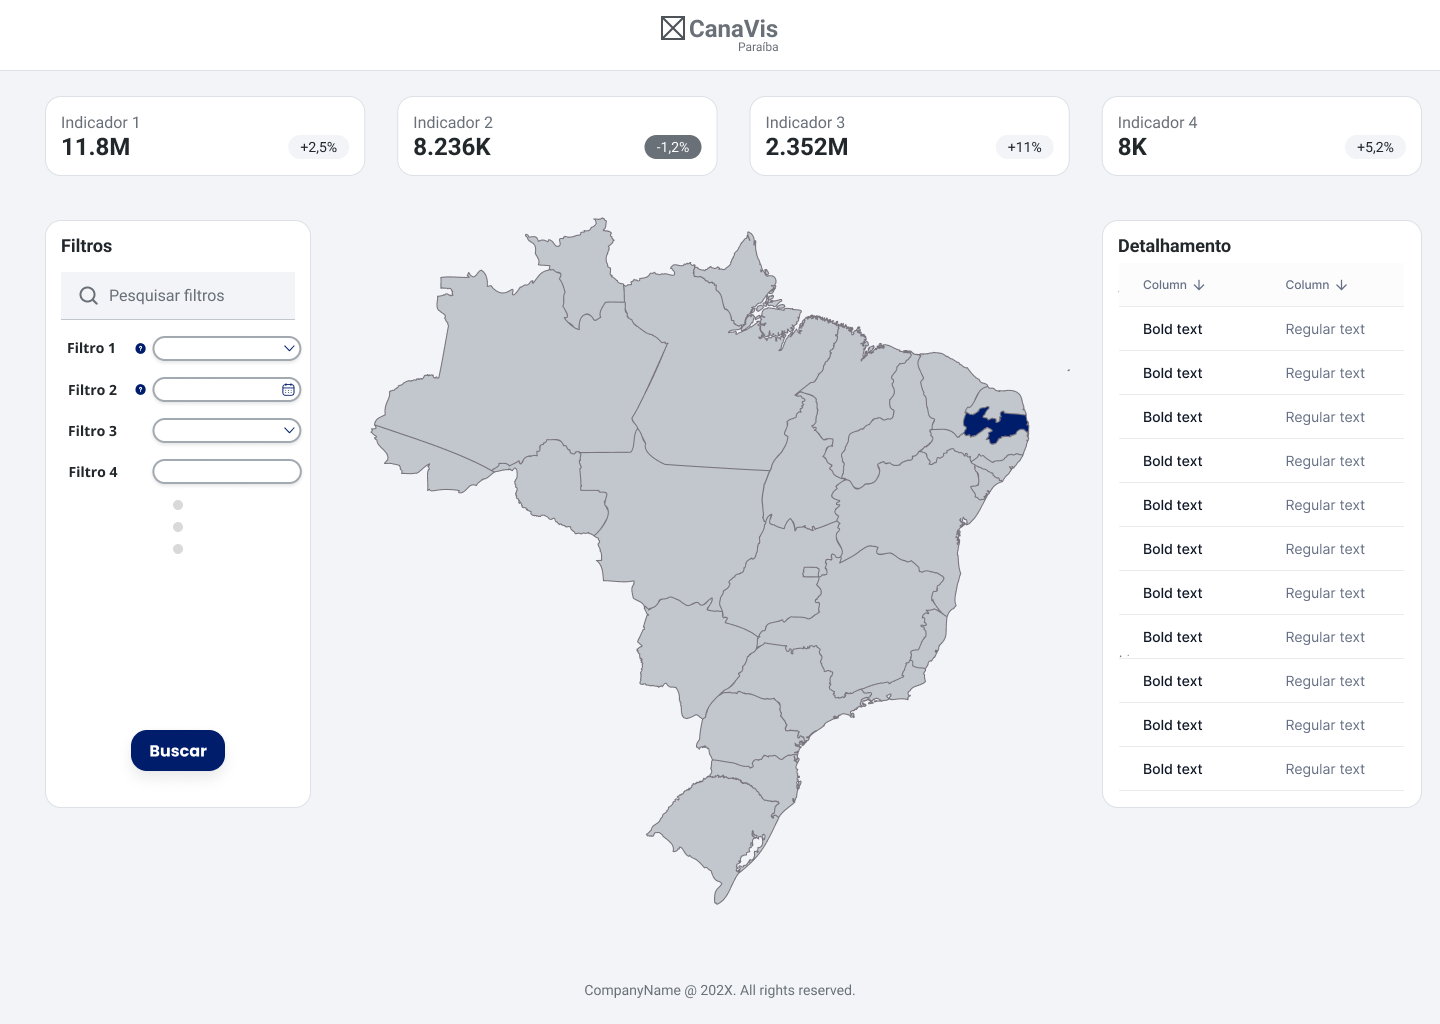
\includegraphics[width=0.32\textwidth]{Layout A.png}\hfill
  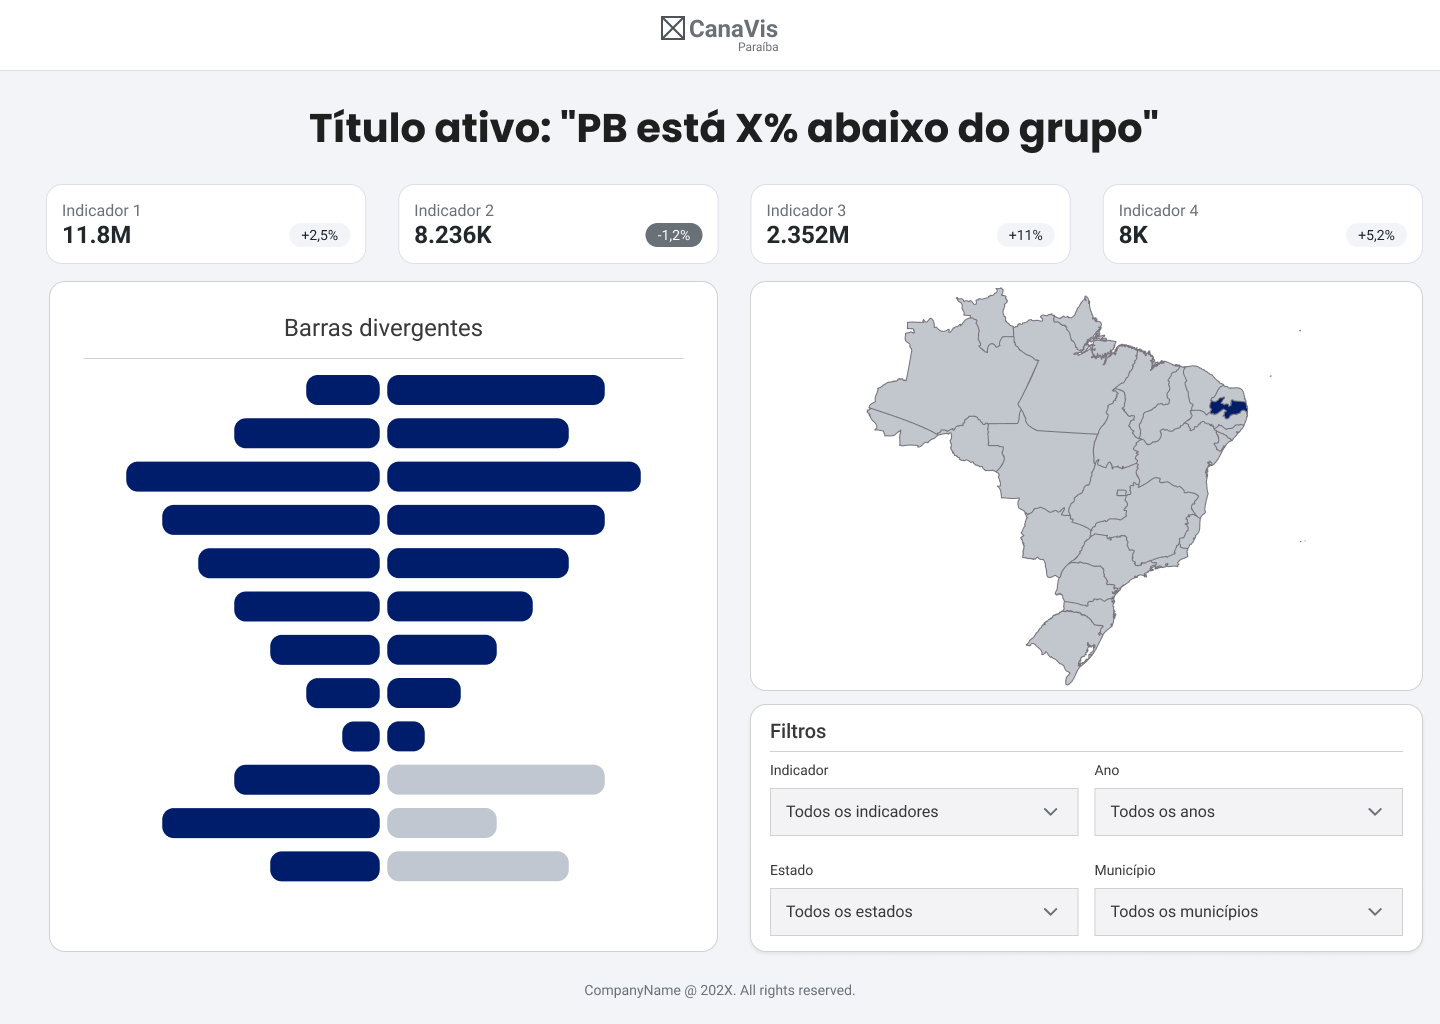
\includegraphics[width=0.32\textwidth]{Layout B.png}\hfill
  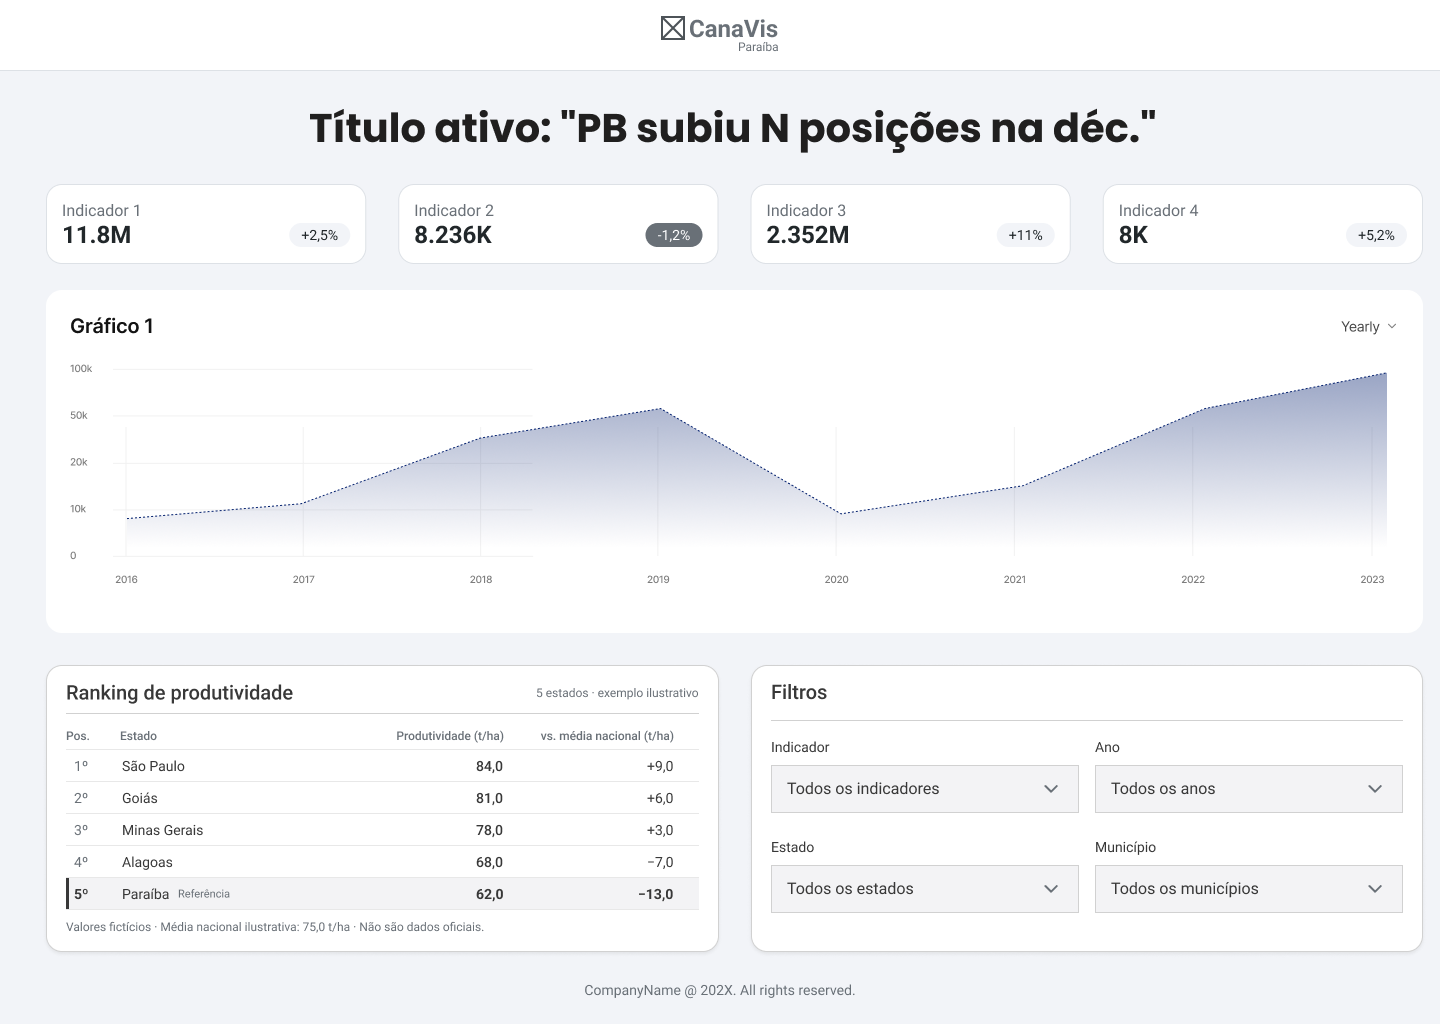
\includegraphics[width=0.32\textwidth]{Layout C.png}
  \caption{Três \textit{layouts} de baixa fidelidade. A (mapa dominante), B (comparação dominante,
  escolhido), C (trajetória dominante). Os descartados foram reaproveitados como telas do fluxo.}
\end{figure}

\begin{longtable}{L{2.4cm} L{5.0cm} L{3.4cm} L{3.4cm}}
\caption{Alternativas de \textit{layout} da tela principal e escolha.}\\
\toprule
\textbf{Layout} & \textbf{Aposta / elemento dominante} & \textbf{O que facilita} & \textbf{O que limita}\\
\midrule
\endfirsthead
\toprule
\textbf{Layout} & \textbf{Aposta} & \textbf{Facilita} & \textbf{Limita}\\
\midrule
\endhead
\bottomrule
\endfoot
A — Mapa & ``Onde estou''; mapa coroplético & Leitura espacial imediata & Cor é fraca para comparar magnitude; não liga à decisão\\
\addlinespace
\textbf{B — Comparação} & ``Acima/abaixo dos pares''; barras divergentes & Posição relativa por comprimento (tarefa precisa) & Perde a geografia (mapa vira apoio)\\
\addlinespace
C — Trajetória & ``Para onde vou''; linha temporal & Evolução ao longo das safras & Dois elementos fortes; pesado para entrada\\
\end{longtable}

\textbf{Escolha: Layout B.} A pergunta principal é de \textit{posicionamento relativo}, e barras
divergentes leem posição por comprimento a partir de uma linha-base comum — a tarefa perceptual
mais precisa, superior à cor do mapa. B torna a comparação o elemento dominante e o mapa um apoio
de contexto, respondendo ao feedback. Para a pergunta mais importante, foram consideradas três
formas visuais, com o que cada uma facilita e esconde:

\begin{longtable}{L{3.2cm} L{4.2cm} L{4.2cm} L{2.6cm}}
\caption{Formas visuais consideradas para a pergunta de posicionamento.}\\
\toprule
\textbf{Forma} & \textbf{Facilita} & \textbf{Esconde / limita} & \textbf{Tarefa}\\
\midrule
\endfirsthead
\toprule
\textbf{Forma} & \textbf{Facilita} & \textbf{Esconde} & \textbf{Tarefa}\\
\midrule
\endhead
\bottomrule
\endfoot
Mapa coroplético & Vizinhança e concentração geográfica & Compara mal valores próximos; achata o pequeno ao lado do grande & Cor (fraca)\\
\addlinespace
\textbf{Barras divergentes} & Posição acima/abaixo da referência, imediata & Perde a geografia; depende da referência escolhida & Comprimento (precisa)\\
\addlinespace
Dot plot / ranking & Ordenação e magnitude com muitas UFs & Não mostra espaço nem evolução & Posição (precisa)\\
\end{longtable}

A \textit{pizza} de participação (mais de três fatias, com 27 UFs) foi descartada explicitamente:
ângulo é tarefa perceptual fraca e o roteiro proíbe pizza com mais de três fatias.

% ==================================================================
\section{Modelo de dados e transformações}

A base tratada é consumida como um modelo estrela de sete tabelas, geradas pelo \textit{pipeline}
do projeto na camada \texttt{processed} (Parquet) e lidas no Power BI pela URL \textit{raw} do
GitHub via \texttt{Web.Contents} — o que torna o modelo portável entre as máquinas do grupo, sem
caminho local embutido.

\textbf{Fato e dimensões.} A tabela de fatos central é \texttt{fato\_producao} (território $\times$
ano $\times$ fonte), acompanhada de \texttt{fato\_industria} (CONAB) e das vendas de etanol da ANP.
As dimensões são \texttt{dim\_territorio} (município, microrregião e UF, distinguidos por
\texttt{nivel\_territorial}), \texttt{dim\_calendario} (contínua, marcada como tabela de datas) e
\texttt{dim\_fonte}. Todas as doze relações são 1:N, com direção de filtro única (da dimensão para
a fato); não há relação fato–fato.

\begin{longtable}{L{3.6cm} L{3.4cm} L{7.4cm}}
\caption{Principais etapas do Power Query.}\\
\toprule
\textbf{Etapa} & \textbf{O que faz} & \textbf{Por que / decisão de tratamento}\\
\midrule
\endfirsthead
\toprule
\textbf{Etapa} & \textbf{O que faz} & \textbf{Por que / decisão}\\
\midrule
\endhead
\bottomrule
\endfoot
\texttt{Web.Contents} & Lê o Parquet da \textit{gold} pela URL \textit{raw} do GitHub & Modelo portável, sem caminho de máquina; mesmo arquivo para todo o grupo\\
\addlinespace
\texttt{Parquet.Document} & Importa com os tipos publicados & Preserva nulos e zeros reais sem conversão textual\\
\addlinespace
Classificação de ausência & Marca valor como \textit{presente}, \textit{sem\_producao} (zero real) ou \textit{suprimido} & A PAM suprime municípios pequenos; suprimido permanece nulo, nunca zero\\
\addlinespace
Alinhamento temporal & Alinha ano civil (IBGE) e safra (CONAB) pela regra do ano inicial & Os calendários diferem; a regra é declarada, não implícita\\
\addlinespace
\textit{Tier} de escala & Lê \texttt{tier} direto do Parquet (preenchido nas 27 UFs) & Agrupa pares de porte semelhante (Seção~\ref{sec:tiers})\\
\end{longtable}

\begin{figure}[H]
  \centering
  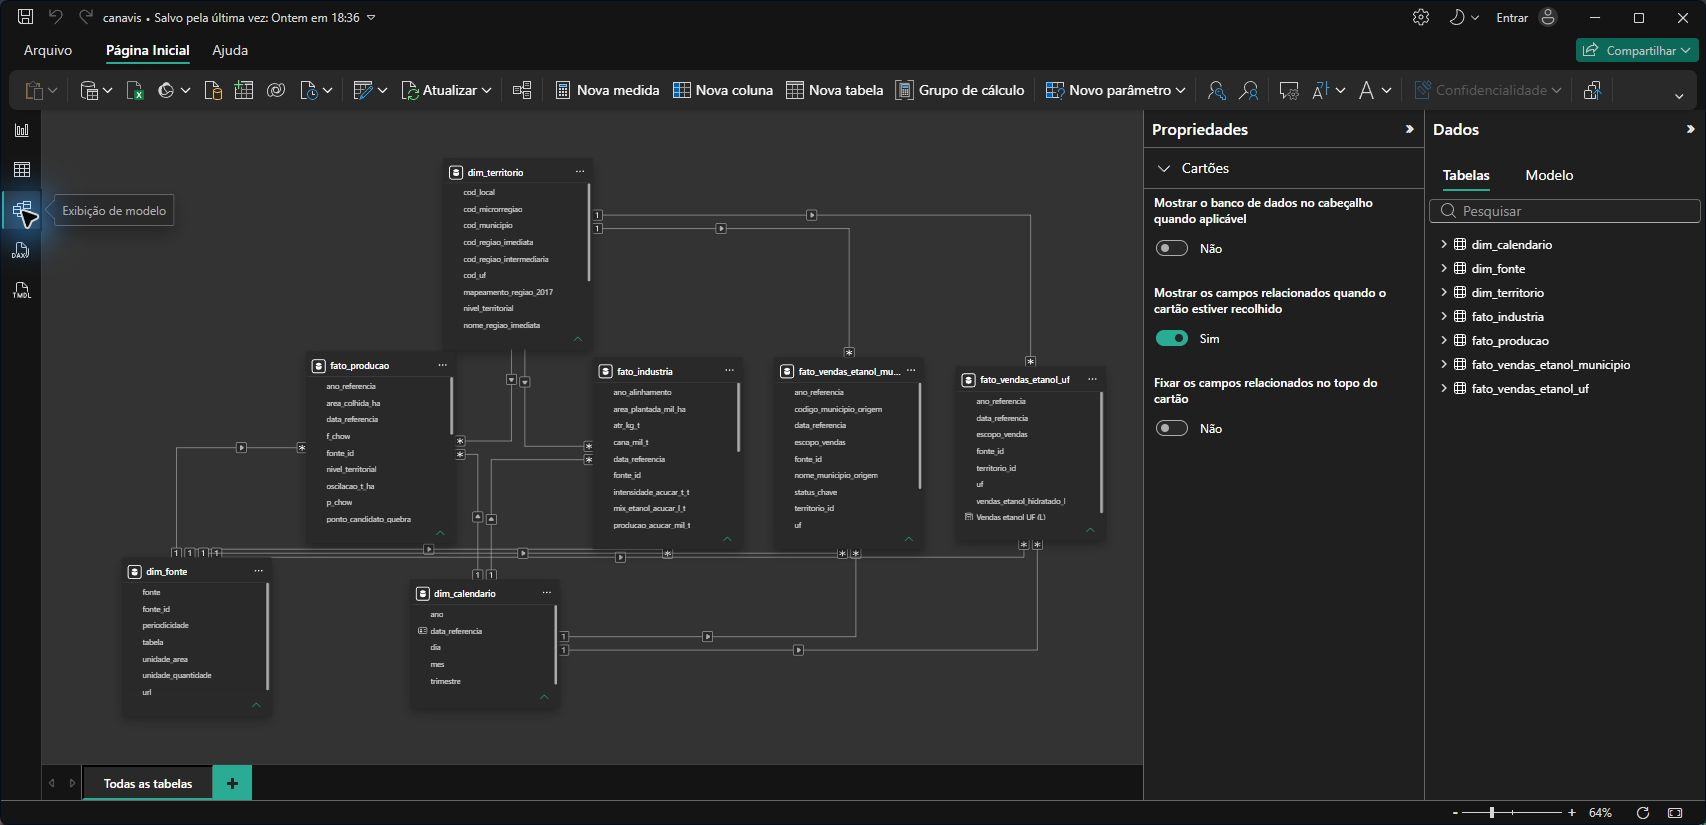
\includegraphics[width=0.92\textwidth]{modelo-integrado.png}
  \caption{Captura da visão de modelo no Power BI: esquema estrela com a fato de produção, as
  fatos industrial e de vendas, e as dimensões de território, calendário e fonte. As doze
  relações são 1:N, com direção de filtro única (da dimensão para a fato).}
\end{figure}

\textbf{Granularidade.} Produtividade é sempre $\sum$quantidade $\div$ $\sum$área, nunca média de
rendimentos (que daria erro de 21,5\%), e exige um único nível territorial no contexto para não
somar totais sobrepostos. Conferência: PB, UF, 2023 $\rightarrow$ 7.066.802 t sobre 109.237 ha
$=$ \textbf{64,69 t/ha}, consistente com a \textit{gold}.

% ==================================================================
\section{Filtros e rotas de navegação}

O relatório tem quatro telas com navegação explícita. A transição obrigatória que transporta
contexto é o \textit{drill-through} do Panorama para o Detalhe do Estado: ao clicar em uma UF, a
tela de destino abre filtrada apenas por ela (p.ex. ``Detalhe de Pará'', com a produtividade do
PA, não o total nacional). Três segmentações relevantes governam o Panorama: Ano, Grupo industrial
(\textit{tier}) e Referência de comparação (o parâmetro da Seção~\ref{sec:cenarios}).

\begin{longtable}{L{3.0cm} L{3.0cm} L{2.6cm} L{2.4cm} L{3.0cm}}
\caption{Tabela 2.1 — Mapa de rotas implementado.}\\
\toprule
\textbf{Origem} & \textbf{Destino} & \textbf{Mecanismo} & \textbf{Contexto} & \textbf{Pergunta que responde}\\
\midrule
\endfirsthead
\toprule
\textbf{Origem} & \textbf{Destino} & \textbf{Mecanismo} & \textbf{Contexto} & \textbf{Pergunta}\\
\midrule
\endhead
\bottomrule
\endfoot
Panorama Nacional & Detalhe do Estado & \textbf{Drill-through} & UF clicada & Como essa UF se posiciona e evoluiu?\\
\addlinespace
Detalhe do Estado & Detalhamento PB & Botão & — (fixo na PB) & Como se distribuem produtividade e vendas nas microrregiões/municípios da PB?\\
\addlinespace
Todas & Metodologia & Botão & — & Fontes, definições e limitações?\\
\addlinespace
Detalhe / PB & Panorama & Botão de voltar & — & Voltar à visão geral\\
\end{longtable}

A transição Estado $\rightarrow$ Município é botão fixo na PB (não \textit{drill-through} com
contexto) porque a base municipal só foi coletada e validada para a Paraíba; as demais UFs só
existem em nível UF. O requisito de transição com contexto já é cumprido por Panorama
$\rightarrow$ Estado.

% ==================================================================
\section{Medidas calculadas em DAX}

Foram criadas medidas (não colunas calculadas); pelo menos uma altera o contexto de filtro, e uma
reproduz um indicador derivado da Etapa 1 (produtividade).

\begin{longtable}{L{3.2cm} L{6.8cm} L{2.4cm} L{2.0cm}}
\caption{Tabela 2.2 — Medidas criadas no Power BI.}\\
\toprule
\textbf{Medida} & \textbf{Expressão / regra DAX} & \textbf{Pergunta} & \textbf{Onde}\\
\midrule
\endfirsthead
\toprule
\textbf{Medida} & \textbf{Expressão DAX} & \textbf{Pergunta} & \textbf{Onde}\\
\midrule
\endhead
\bottomrule
\endfoot
Produtividade & \texttt{DIVIDE(SUM(quantidade), SUM(area))}, com nível único e sem parcela nula & Quanto se produz por hectare? & Cartões, ranking\\
\addlinespace
Participação regional & Razão sobre o total do nível; \texttt{CALCULATE}/\texttt{ALL} troca o denominador & Quanto o território pesa no total? & Panorama\\
\addlinespace
Desvio vs seleção & \texttt{CALCULATE([Produtividade], ALLSELECTED(dim\_territorio))} como referência & Quanto difere do conjunto selecionado? & Panorama\\
\addlinespace
Desvio vs grupo & Referência com \texttt{ALLSELECTED} e \texttt{KEEPFILTERS(tier = Tier)} & Quanto difere dos pares de porte? & Panorama (cenário)\\
\end{longtable}

As medidas protegem contra ausência: se uma parcela de quantidade ou área estiver suprimida, o
agregado fica vazio em vez de apresentar um total parcial como completo, e o desvio verifica
\texttt{ISBLANK} antes de subtrair (evita ler ausência como $-100\%$). Além destas, o modelo traz
medidas industriais (mix etanol/açúcar e ATR ponderado pela cana) e de vendas.

\textbf{Código DAX completo das medidas obrigatórias.} A produtividade reproduz o indicador da
Etapa 1; o desvio vs.\ grupo altera o contexto de filtro (\texttt{ALLSELECTED}, \texttt{KEEPFILTERS}).

{\footnotesize
\begin{verbatim}
Produtividade =
IF(
  HASONEVALUE(dim_territorio[nivel_territorial])
  && COUNTROWS(FILTER(fato_producao,
       ISBLANK(fato_producao[quantidade_produzida_t])
       || ISBLANK(fato_producao[area_colhida_ha]))) = 0,
  DIVIDE(SUM(fato_producao[quantidade_produzida_t]),
         SUM(fato_producao[area_colhida_ha])))

Desvio vs grupo =
VAR Tier = SELECTEDVALUE(dim_territorio[tier])
VAR Atual = [Produtividade]
VAR Referencia =
    CALCULATE([Produtividade], ALLSELECTED(dim_territorio),
              KEEPFILTERS(dim_territorio[tier] = Tier))
RETURN
    IF(NOT ISBLANK(Tier) && NOT ISBLANK(Atual) && NOT ISBLANK(Referencia),
       DIVIDE(Atual - Referencia, Referencia))
\end{verbatim}
}

% ==================================================================
\section{Parâmetro e cenários alternativos}\label{sec:cenarios}

O parâmetro é de \textit{campo}: troca contra qual referência a produtividade da PB é lida. Ele
muda a \textit{leitura}, não apenas o número — o mesmo 64,69 t/ha conta histórias opostas conforme
a referência.

\begin{longtable}{L{2.4cm} L{3.4cm} L{1.8cm} L{6.4cm}}
\caption{Tabela 2.3 — Cenários simulados (ano 2023).}\\
\toprule
\textbf{Cenário} & \textbf{Parâmetro} & \textbf{PB} & \textbf{Leitura e implicação para a persona}\\
\midrule
\endfirsthead
\toprule
\textbf{Cenário} & \textbf{Parâmetro} & \textbf{PB} & \textbf{Leitura e implicação}\\
\midrule
\endhead
\bottomrule
\endfoot
Base & Desvio vs seleção (27 UFs) & $-16{,}96\%$ & ``Abaixo da média nacional'' — mas a média é puxada por SP (56,8\% da produção). Contexto amplo, pouco acionável.\\
\addlinespace
Alternativo 1 & Desvio vs grupo (\textit{tier} média escala) & $+3{,}41\%$ & A leitura \textbf{inverte de sinal}: entre pares de porte, a PB está acima. Sustenta meta e priorização realistas.\\
\addlinespace
Alternativo 2 & Participação regional & $0{,}90\%$ & Peso da PB no total do país. Separa escala de eficiência — porte e desempenho são perguntas distintas.\\
\end{longtable}

O título ativo do Panorama acompanha a troca (``PB está 3,4\% acima do seu grupo industrial''). É
a resposta direta ao feedback da Etapa 1 sobre ligar a referência à decisão.

% ==================================================================
\section{Narrativa em tela e justificativa visual}

Cada tela tem um título ativo que enuncia a conclusão (não o assunto), um visual dominante e até
dois secundários, e uma linha de contexto com fonte, período e unidade. A escolha de cada gráfico
parte da pergunta analítica da Etapa 1, pela tarefa perceptual exigida:

\begin{itemize}
  \item \textbf{Barras divergentes} (Panorama, dominante) — posicionamento relativo lido por
  comprimento a partir da referência; a tarefa mais precisa para ``acima/abaixo''.
  \item \textbf{Mapa coroplético} (Panorama, secundário) — situa no espaço; cor é fraca para
  magnitude, por isso é apoio, não protagonista.
  \item \textbf{Linha temporal} (Detalhe do Estado) — evolução por inclinação ao longo do tempo.
  \item \textbf{Ranking ordenado} (tabela) — magnitude com ordenação intencional por valor.
  \item \textbf{Barras de top municípios} (Detalhamento PB) — comparação de magnitude a partir do
  zero.
\end{itemize}

\begin{figure}[H]
  \centering
  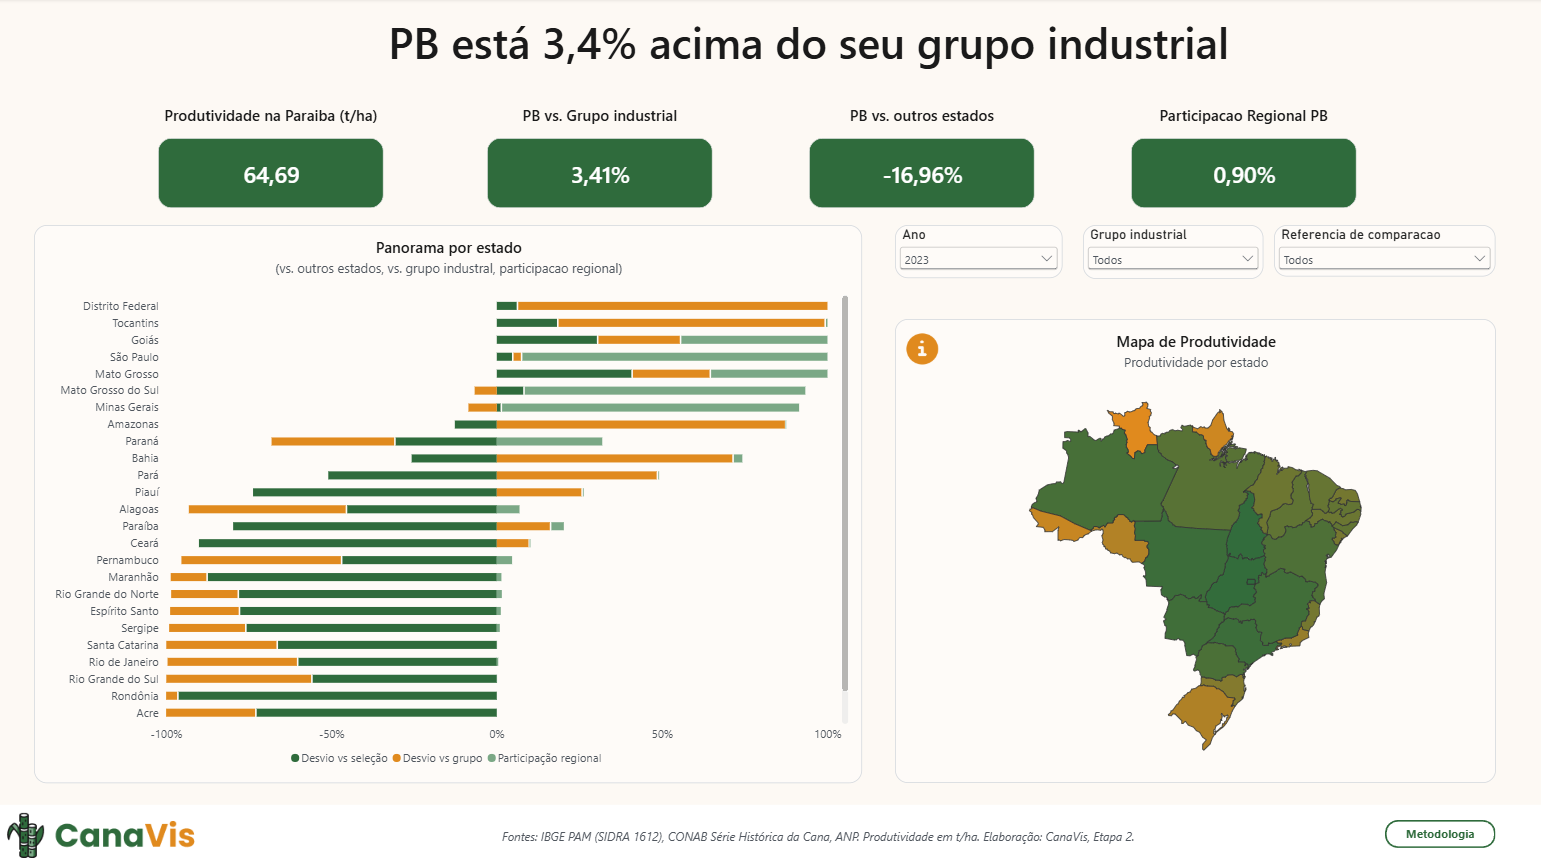
\includegraphics[width=0.85\textwidth]{Panorama Nacional.png}
  \caption{Tela principal (Panorama Nacional): barras divergentes dominantes, mapa de apoio,
  cartões e segmentações. Título ativo enuncia a conclusão.}
\end{figure}

\begin{figure}[H]
  \centering
  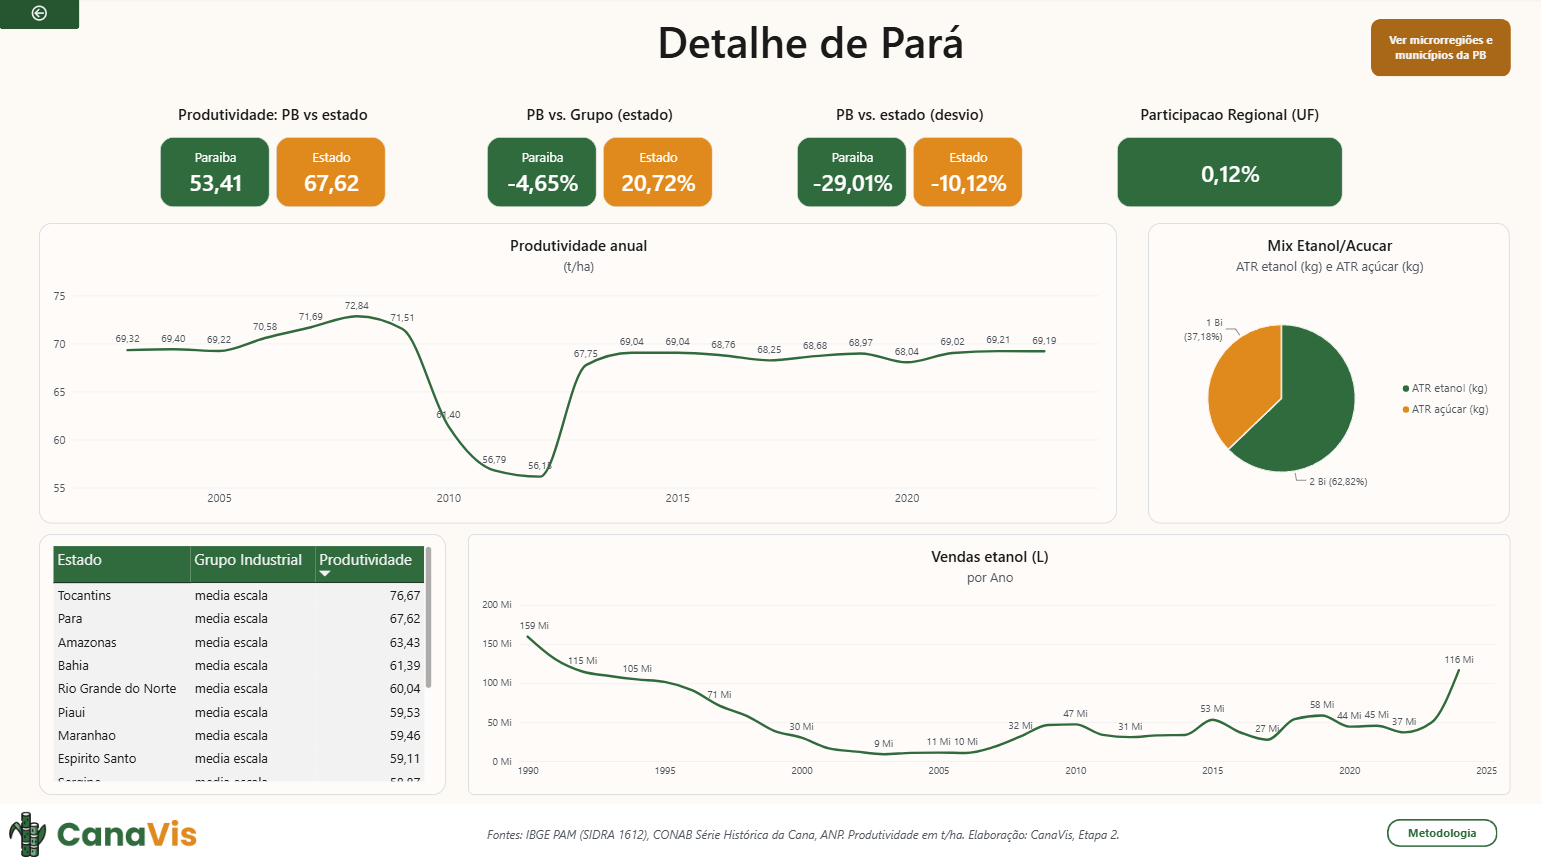
\includegraphics[width=0.85\textwidth]{Detalhe do estado.png}
  \caption{Detalhe do Estado, destino do \textit{drill-through}: série temporal, ranking e mix,
  com os cartões diferenciando o valor da PB do estado selecionado.}
\end{figure}

\textbf{Higiene visual e acessibilidade.} Paleta de cinco cores de dado, com par divergente
verde-cana $\times$ âmbar (não verde $\times$ vermelho, inseguro para daltônicos); contraste do
texto sobre fundo claro acima de 5:1; ordenação por valor, nunca alfabética; sem eixos truncados
sem aviso, sem 3D; a única pizza (mix) tem duas fatias, dentro do limite. Todo indicador exibe
unidade, período e fonte. Uma página de Metodologia reúne fontes, definições e limitações.

% ==================================================================
\section{Comparação por pares: \textit{tiers} de escala}\label{sec:tiers}

O feedback pediu comparação com pares de características semelhantes. As 27 UFs foram agrupadas por
escala de produção (eixo físico: quantidade), por cortes em $\log$ da quantidade — e não por
K-means, porque o diagnóstico mostrou escala praticamente unidimensional (correlação
quantidade$\times$área $= 1{,}000$), distribuição log-normal e concentração extrema (SP sozinho
$=56{,}8\%$). A dispersão de escala intra-grupo caiu 66\% frente à base inteira, e o resultado foi
validado contra agrupamento hierárquico. Os grupos: \textbf{grande escala industrial} (8 UFs,
incl. SP, MG, GO, PR), \textbf{média escala} (14 UFs, onde está a \textbf{Paraíba}) e
\textbf{pequena/marginal} (5 UFs). O agrupamento usa um eixo (escala) e a comparação usa outro
(eficiência), evitando circularidade.

% ==================================================================
\section{Teste com usuário}

O protótipo foi apresentado à persona (gerente agrícola, externa à equipe), com 60 segundos de
observação silenciosa. Ele olhou primeiro os cartões e o título do Panorama, depois o mapa; teve
dificuldade para perceber que o mapa é navegável; na segunda tela navegou com facilidade;
confirmou a veracidade dos dados; e sentiu falta de dados por usina (privados, fora do escopo
público).

\begin{longtable}{L{4.8cm} L{4.6cm} L{4.6cm}}
\caption{Tabela 2.4 — Achados do teste e correções implementadas.}\\
\toprule
\textbf{Observação do usuário} & \textbf{Diagnóstico} & \textbf{Mudança implementada}\\
\midrule
\endfirsthead
\toprule
\textbf{Observação} & \textbf{Diagnóstico} & \textbf{Mudança}\\
\midrule
\endhead
\bottomrule
\endfoot
Não percebeu que o mapa é navegável & A navegação por \textit{drill-through} não se anuncia & Ícone informativo com \textit{tooltip} no mapa do Panorama\\
\addlinespace
Não distinguia valor da PB do estado nos cartões & Dois valores sem rótulo de identificação & Novo \textit{layout} dos cartões rotulando ``Paraíba'' e ``Estado''\\
\addlinespace
Procurou a metodologia; rótulos desalinhados & Acesso não uniforme; ruído visual & Botão de Metodologia em todas as telas e alinhamento dos rótulos\\
\end{longtable}

O comentário sobre preços internacionais e câmbio não virou mudança nesta etapa: é caminho já
mapeado para a Etapa 3, e o próprio feedback da Etapa 1 alertou contra ampliar escopo sem
diagnóstico de fontes.

% ==================================================================
\section{Discussão}

\textbf{(i) O que da Etapa 1 não sobreviveu aos dados.} A \textit{quebra estrutural} da série de
produtividade não se confirmou: com 21 pontos anuais, o teste de Chow endógeno recai em 2013 mas
fica abaixo do crítico, e a PB não sobrevive à correção de múltiplas comparações (p ajustado
0,0606). A tela passou a \textit{descrever} queda e recuperação, nunca a \textit{afirmar} quebra.
O ranking municipal de tendência caiu por supressão (62\% no município). E a comparação nacional
crua se mostrou enganosa — daí os \textit{tiers}.

\textbf{(ii) Limitações do Power BI e caminho da Etapa 3.} A decomposição tendência/oscilação está
calculada e materializada, mas sua \textit{exibição} foi adiada: numa série tão curta, mostrar
tendência e banda de incerteza pode comunicar mais certeza do que os dados permitem — será
validada com o professor e levada à Etapa 3, junto de fontes de horizonte mais longo (preço e
câmbio). A Etapa 3, em Dash, consome a mesma camada \texttt{processed} e permite controle fino que
o Power BI não oferece.

\textbf{(iii) O que falta para ser útil à persona.} Dados por usina (privados), preços e câmbio
(demanda do teste e do feedback) e séries mais longas. O produto cumpre hoje o núcleo da decisão —
situar a produtividade da região frente aos pares — e deixa esses caminhos para a próxima etapa,
cada um condicionado a diagnóstico de fonte, como o feedback exigiu.

\end{document}
